\section{Medición y error experimental}

\subsection{Objetivos}
\begin{itemize}
	\item Determinar las condiciones para que un péndulo simple tenga su período independiente de su amplitud angular.
	\item Determinar la relación entre el período y la longitud l del péndulo.
	\item Construir funciones polinómicas que representen a dicha función.
\end{itemize}
\subsection{Fundamento Teórico}
\begin{itemize}
	\item \textbf{Período (T):}

	      El período mide el tiempo que se tarde en dar una vuelta completa y se mide en segundos.
	      La unidad del periodo en el S.I. es el segundo(s).
	\item \textbf{Frecuencia (f) :}

	      La frecuencia mide la cantidad de vueltas que se dan en un período de tiempo. La unidad de
	      la frecuencia en el S.I. es el Hertz($s^-1$).
	      \begin{equation*}
		      f=\dfrac{N^{\circ} \text { ciclos }}{t}=\dfrac{1}{T}
	      \end{equation*}
	\item \textbf{Frecuencia angular($w$):}
	      Se refiere a la frecuencia del movimiento circular expresada en proporción del cambio de
	      ángulo, y se define como veces la frecuencia. Se expresa en radianes/Segundo, y formalmente,
	      se define con la letra omega minúscula($w$) a través de la fórmula:
	      \begin{equation*}
		      w=2\pi f=\dfrac{2\pi}T
	      \end{equation*}
	\item \textbf{Osilaciones :}
	      Se dice que es una variación, perturbación o fluctuación en el tiempo de un medio o sistema. Si
	      el fenómeno se repite, se habla de oscilación periódica.
	      Una oscilación, en física, química e ingeniería es el movimiento repetido de un lado a otro en
	      torno a una posición central, o posición de equilibrio. El recorrido que consiste en ir desde una
	      posición extrema a la otra y volver a la primera, pasando dos veces por la posición central, se
	      denomina ciclo. El número de ciclos por segundo, Hertz (Hz), se conoce como frecuencia de la
	      oscilación empleada en el movimiento armónico simple.
	\item \textbf{Movimiento Armónico Simple:}
	      Hay muchas situaciones en física en las cuales la fuerza que siente una partícula en cierto
	      sistema es proporcional a un desplazamiento respecto cierto punto “de equilibrio”. Es decir,
	      existen sistemas para los cuales es válida la ley de Hooke.
	      \begin{equation*}
		      F = -kx
	      \end{equation*}
	\item \textbf{Péndulo:}
	      Existen muy variados tipos de péndulos que, atendiendo a su configuración y usos,
	      reciben los nombres apropiados: péndulo simple, péndulo compuesto, péndulo cicloidal,
	      doble péndulo, péndulo de Foucault, péndulo de Newton, péndulo balístico, péndulo de
	      torsión, péndulo esférico, etcétera.
	\item \textbf{Péndulo Simple}
	      El péndulo simple es un sistema mecánico que se mueve en un movimiento oscilatorio.
	      Un péndulo simple se compone de una masa puntual m suspendida por una cuerda
	      ligera supuestamente inextensible de longitud l, donde el extremo superior de la cuerda
	      está fijo
\end{itemize}
\subsection{Materiales y  equipos de trabajo}
\begin{figure}[H]
	\begin{center}
		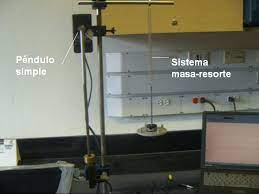
\includegraphics[width = 0.5\textwidth]{Imagenes/pen.jpg}
		\captionof{figure}{pendulo simple}
	\end{center}
\end{figure}

\begin{figure}[H]
	\begin{center}
		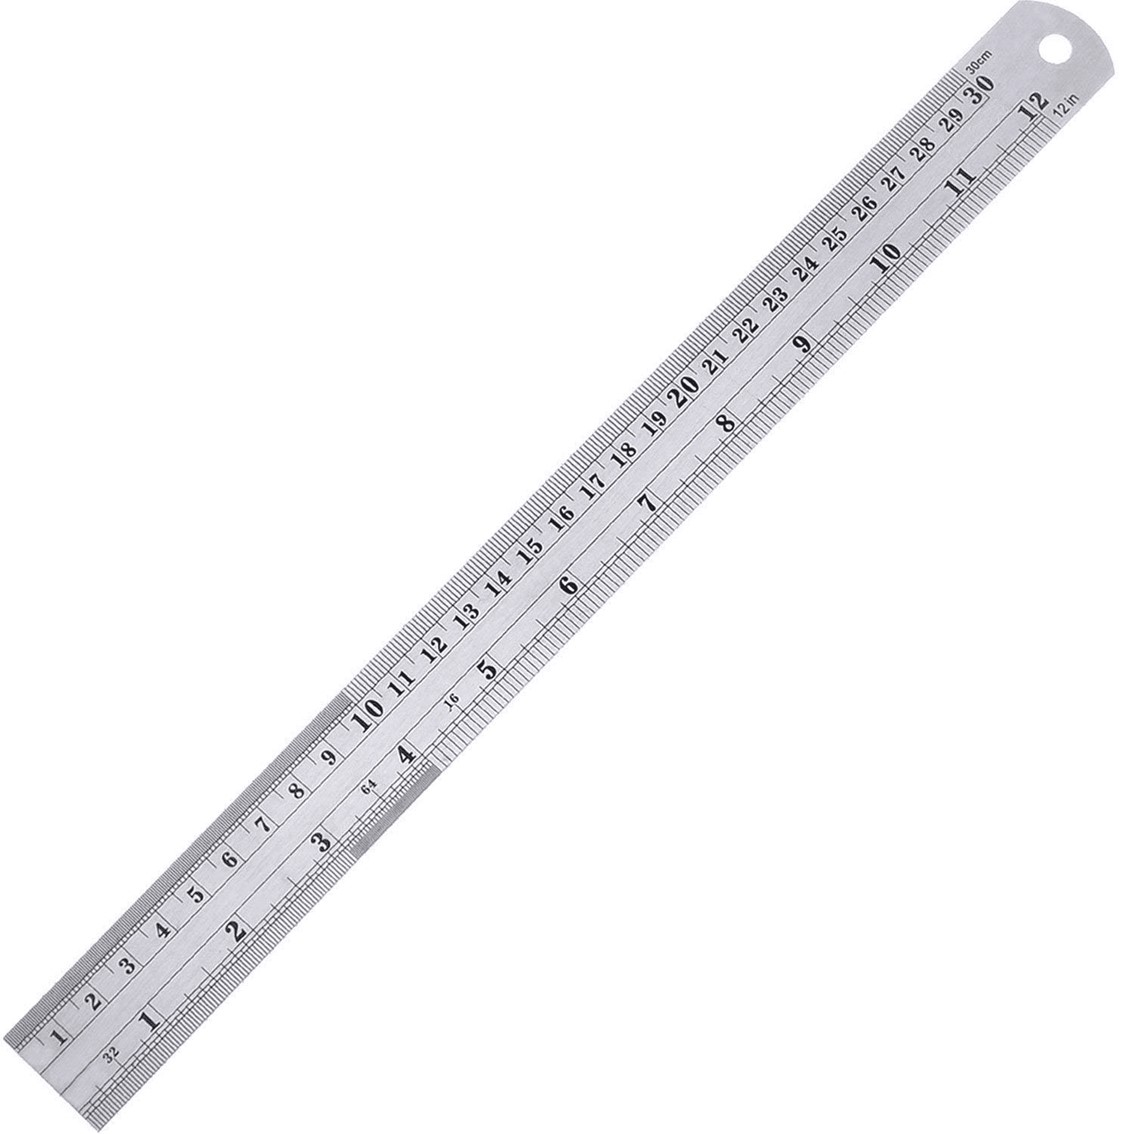
\includegraphics[width = 0.5\textwidth]{Imagenes/regla.jpg}
		\captionof{figure}{una regla}
	\end{center}
\end{figure}

\begin{figure}[H]
	\begin{center}
		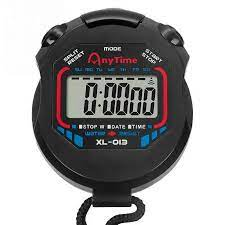
\includegraphics[width = 0.4\textwidth]{Imagenes/crono.jpg}
		\captionof{figure}{un cronometro}
	\end{center}
\end{figure}

\subsection{Procedimientos}
\begin{enumerate}
	\item  Tome la pieza metálica y con la regla, mida tres veces y en lugares diferentes, el largo, el ancho, el alto, el diámetro mayor y el diámetro menor de los agujeros de la pieza.
	\item Tome la pieza metálica y con el pie de rey, mida tres veces y en lugares diferentes, el largo, el ancho, el alto, el diámetro mayor, el diámetro menor, la altura mayor del agujero y la altura menor del agujero.
	\item Determine la incertidumbre de la regla y del pie de rey.
	\item Con las mediciones realizadas y sus incertidumbres, calcule el  área lateral (es decir la suma de las áreas de las caras donde no está el agujero) de la pieza con su incertidumbre respectiva.

\end{enumerate}
\subsection{Resultados Obtenidos}


\begin{xltabular}{\textwidth}{|c|c|}
	\caption{Tabla de Incertidumbre humana} \\

	\hline \multicolumn{1}{|c|}{\textbf{Activación del cronómetro}} & \multicolumn{1}{c|}{\textbf{Tiempo}}  \\ \hline
	\endfirsthead

	\multicolumn{2}{c}%
	{} \\
	\hline
	\endhead

	\hline \multicolumn{2}{|r|}{{Continued on next page}} \\ \hline
	\endfoot

	\hline
	\endlastfoot
	1                         & 0,23                         \\
	2                         & 0,2                          \\
	3                         & 0,18                        \\
	4                         & 0,21                         \\
	5                         & 0,18                         \\
	6                         & 0,15                         \\ \hline
	Promedio (incertidumbre)  & 0,19
\end{xltabular}



\begin{xltabular}{\textwidth}{|c|c|c|c|c|c|c|c|}
	\caption{Tabla de resultados de medición del Periodo} \\

	\hline \multicolumn{1}{|c|}{K} & \multicolumn{1}{c|}{\textbf{L(cm)}} & \multicolumn{1}{c|}{\textbf{$T_1$}} & \multicolumn{1}{c|}{\textbf{$T_2$}} & \multicolumn{1}{c|}{\textbf{$T_3$}} & \multicolumn{1}{c|}{\textbf{$T_4$}} & \multicolumn{1}{c|}{\textbf{$T_k$}} & \multicolumn{1}{c|}{\textbf{($T_k)^2$}}  \\ \hline
	\endfirsthead

	\multicolumn{8}{c}%
	{} \\
	\hline
	\endhead

	\hline \multicolumn{8}{|r|}{{Continued on next page}} \\ \hline
	\endfoot

	\hline
	\endlastfoot
	1          & 20     & 0,961   & 0,964  & 0,949  & 0,95   & 0,956  & 0,914 \\
	2          & 30     & 1,233   & 1,234  & 1,236  & 1,222  & 1,231  & 1,515 \\
	3          & 40     & 1,343   & 1,345  & 1,347  & 1,34   & 1,34   & 1,796 \\
	4          & 50     & 1,472   & 1,475  & 1,486  & 1,49   & 1,48   & 2,190 \\
	5          & 60     & 1,598   & 1,595  & 1,601  & 1,594  & 1,59   & 2,528 \\
	6          & 70     & 1,716   & 1,725  & 1,721  & 1,724  & 1,72   & 2,958 \\
	7          & 80     & 1,847   & 1,84   & 1,834  & 1,838  & 1,83   & 3,349 \\
	8          & 90     & 1,947   & 1,934  & 1,93   & 1,932  & 1,94   & 3,764 \\
	9          & 100    & 2,042   & 2,037  & 2,031  & 2,031  & 2,04   & 4,162
\end{xltabular}


\textbf{Representación polinómica de los resultados Método:} Ajuste lineal por mínimos cuadrados




\begin{enumerate}
	\item Preparación de los valores implicados en la operación







	      \begin{xltabular}{\textwidth}{|c|c|c|c|c|c|c|c|}
		      \caption{Tabla de resultados de medición del Periodo} \\

		      \hline \multicolumn{1}{|c|}{} & \multicolumn{1}{c|}{\textbf{x}} & \multicolumn{1}{c|}{\textbf{y}} & \multicolumn{1}{c|}{\textbf{$xy$}} & \multicolumn{1}{c|}{\textbf{$x^2$}} & \multicolumn{1}{c|}{\textbf{$y^2$}}   \\ \hline
		      \endfirsthead

		      \multicolumn{6}{c}%
		      {} \\
		      \hline
		      \endhead

		      \hline \multicolumn{6}{|r|}{{Continued on next page}} \\ \hline
		      \endfoot

		      \hline
		      \endlastfoot
		      & 20  & 0,914  & 18,28   & 400,000   & 0,835  \\
		      & 30  & 1,515  & 45,45   & 900,000   & 2,295  \\
		      & 40  & 1,796  & 71,84   & 1600,000  & 3,226  \\
		      & 50  & 2,190  & 109,5   & 2500,000  & 4,796  \\
		      & 60  & 2,528  & 151,68  & 3600,000  & 6,391  \\
		      & 70  & 2,958  & 207,06  & 4900,000  & 8,750  \\
		      & 80  & 3,349  & 267,92  & 6400,000  & 11,216 \\
		      & 90  & 3,764  & 338,76  & 8100,000  & 14,168 \\
		      & 100 & 4,162  & 416,2   & 10000,000 & 17,322 \\ \hline
		      Sumatorias         & 540 & 23,176 & 1626,69 & 38400,000 & 68,999 \\  \hline
		      Media              & 60  & 2,575 & & &
	      \end{xltabular}

	\item Operciones

	      \begin{equation*}
		      m=\dfrac{n\left(\sum x y\right)-\left(\sum x\right)\left(\sum y\right)}{n\left(\sum x^2\right)-\left(\sum x\right)^2}=0,0394
	      \end{equation*}
	      \begin{equation*}
		      b=\bar{y}-m \bar{x}=0,2138
	      \end{equation*}
	      \begin{equation*}
		      r=\dfrac{n\left(\sum x y\right)-\left(\sum x\right)(\Sigma y)}{\sqrt{\left[n\left[\sum x^2\right)-\left(\sum x\right)^2\right]\left[n\left(\Sigma y^2\right)-(\Sigma y)^2\right]}}=0,9987
	      \end{equation*}
	      \begin{equation*}
		      r^2=(\dfrac{n\left(\sum x y\right)-\left(\sum x\right)(\Sigma y)}{\sqrt{\left[n\left[\sum x^2\right)-\left(\sum x\right)^2\right]\left[n\left(\Sigma y^2\right)-(\Sigma y)^2\right]}})^2=0,9973
	      \end{equation*}

	      \textbf{Entonces la Ecuación de la recta hallada es : $y = 0,03935x + 0,21381$}
	\item De la ecuacion se obtiene y superponiendo las mediciones reales

	      \begin{figure}[H]
		      \begin{center}
			      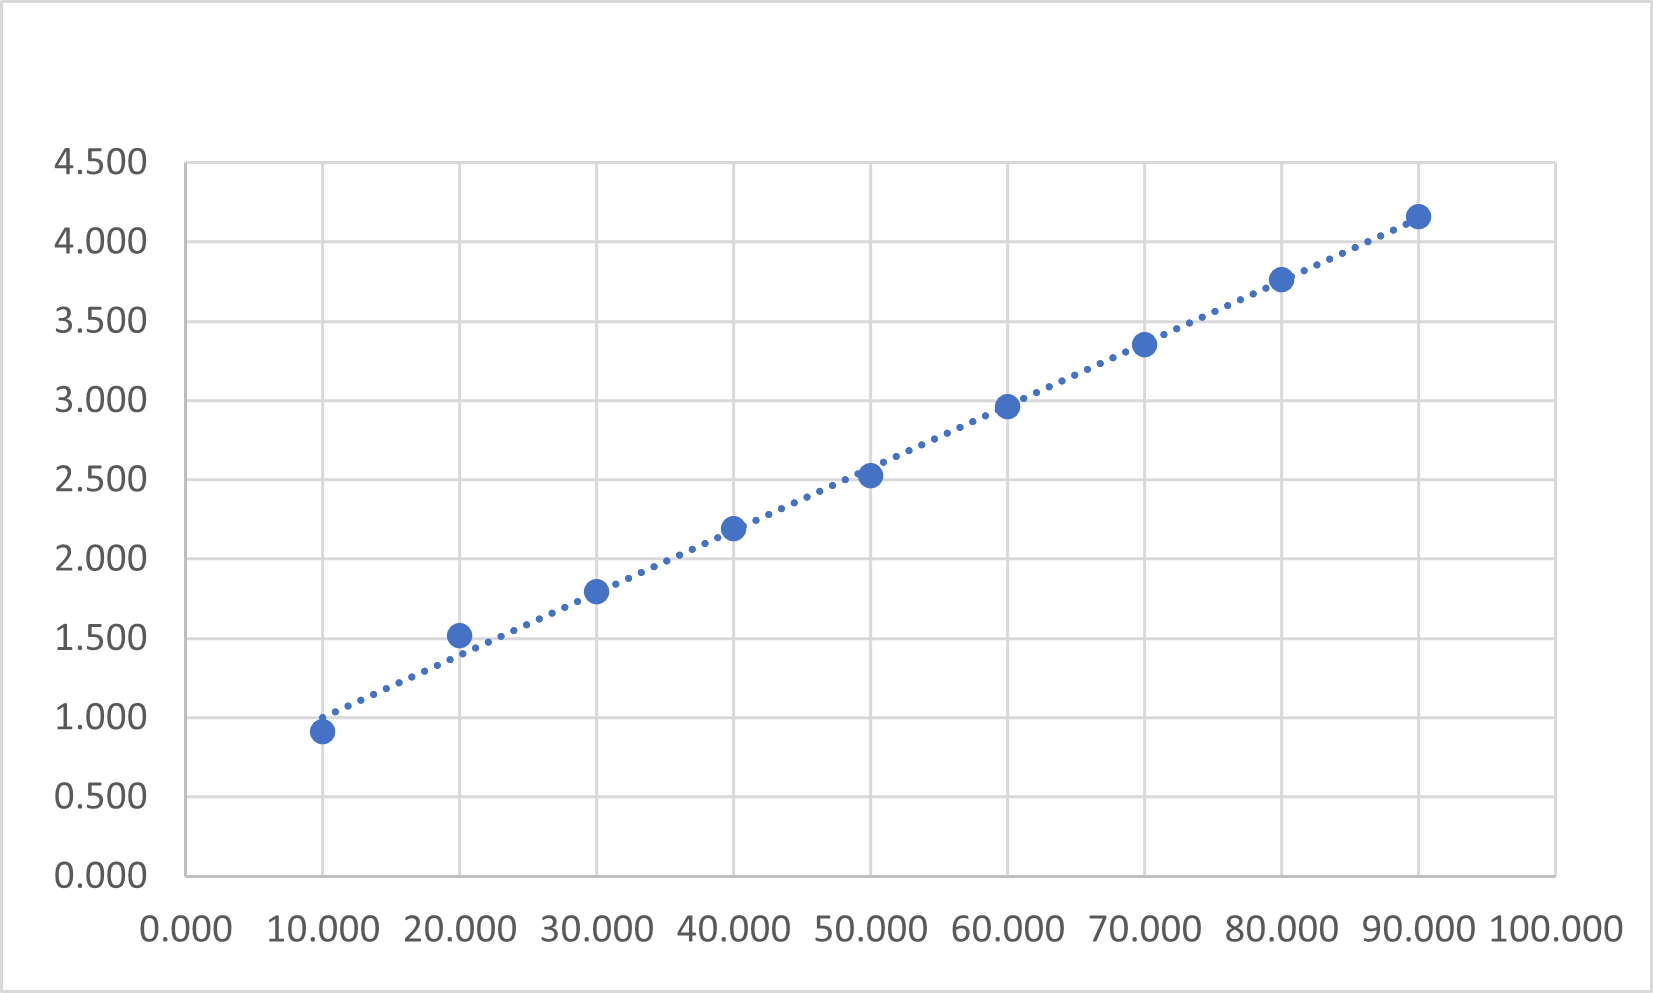
\includegraphics[width = 0.6\textwidth]{Imagenes/Imagen3.png}
			      \captionof{figure}{ del periodo al cuadrado en funcion de la longitud}
		      \end{center}
	      \end{figure}
\end{enumerate}

\subsection{Cuestionario}
\begin{enumerate}
	\item \textbf{Anteriormente se le ha pedido que para medir el periodo suelte la masa del péndulo. ¿Qué sucede si en vez de ello lanza la masa?}

	      Si se lanza la masa, se tendría una aceleración inicial que alteraría considerablemente el periodo de oscilación a medir.
	\item \textbf{¿Depende el per\'iodo del tamaño que tenga la masa? Explique.}


	      Una masa de mayor tamaño no representaría un cambio apreciable a la medición del periodo a pesar de la resistencia del aire, siendo esta mínima. Incluso si se desprecia la resistencia del aire, el periodo sería totalmente independiente del objeto.
	\item \textbf{Para determinar el periodo (duración de una oscilacion completa), se ha pedido medir la duración de 10 oscilaciones y de allí determinar la duración de una oscilación. ¿Por qué no es conveniente medir la duración de una sola oscilación? ¿Qué sucedería si midiera el tiempo necesario para 50 oscilaciones?}
	      \begin{itemize}
		      \item Primero, no es conveniente medir una única oscilación debido al error humano por el tiempo de reacción, mientras que con 10 oscilaciones es posible predecir el fin de una oscilación y así minimizar el error.
		      \item Segundo, podría haber más exactitud en la medición pero es más probable que no llegue a las 50 oscilaciones debido a la resistencia del aire y a eso se podría añadir la fatiga humana de medir 50 oscilaciones por repetición.
	      \end{itemize}

	\item \textbf{¿Cuantas oscilaciones cree que daria el péndulo de longitud 100 cm antes de detenerse?}
	      Aproximadamente unas 40 oscilaciones antes de detenerse
	\item \textbf{Observe que al soltar el p\'endulo es muy dif\'icil evitar que la masa “rote” ¿Modifica tal rotaci\'on el valor del periodo?}
	      Va a modificar el valor del periodo medido porque añade momentum extra, sin embargo esa variación sería despreciable.

\end{enumerate}
\subsection{observaciones}
\begin{enumerate}
	\item Con respecto a la medición de la pieza metálica debemos tomar en cuenta no solo la incertidumbre y el error humano, sino también la forma y disposición de la mesa donde se realiza la medición. por ejemplo sus imperfecciones, como muescas, rayones y deformaciones que pueden afectar los resultados.
	\item La medición de la longitud de la cuerda del péndulo se ve afectada en cierta medida por la elasticidad del material, no solo por la incertidumbre en los instrumentos y el error humano
	\item Las diferentes formas en que se realiza el nudo afectan también a la longitud final del péndulo, ya sea por el ángulo en que se realice o que tan ajustado sea el nudo
	\item la propia masa usada también puede contribuir a la imprecisión debido a que no es una pieza sólida, sino más bien dos piezas unidas que pueden tener algo de movimiento respecto una a la otra (sin embargo es despreciable)
	\item debido a factores como externos como la poca familiaridad con el laboratorio, la programación de un evento que mantenía cierta presión en el horario (la fumigación del laboratorio) e incomodidad general por las alta temperatura, podría verse afectada de forma negativa la capacidad de los participantes para tomar las medidas de forma precisa y consistente.
	\item Los movimientos de los participantes pueden afectar al movimiento del péndulo y a la precisión de las mediciones de la pieza metálica

\end{enumerate}
\subsection{Conclusiones}
\begin{itemize}
	\item Aprender a realizar mediciones de forma precisa y tomando en cuenta tanto la incertidumbre como el error humano es muy importante para estudios científicos debido a que es la base de cualquier experimento.
	\item La manipulación de los instrumentos de medición debe realizarse con cuidado para evitar daños y deformaciones que puedan alterar las mediciones a futuro. Incluso, aunque estas variaciones sean mínimas, al momento de operar resultará en errores más grandes.
	\item La comunicación es sumamente importante al momento de coordinar quienes realizan la experimentación y quienes registrarán los resultados, y cuales son los parámetros base de la experiencia.
	\item Antes de la realización del experimento es necesario revisar los materiales a usar y las distintas situaciones y variaciones que estos puedan experimentar. Casos como el uso de una cuerda muy elástica, una mesa irregular, o instrumentos dañados deben evitarse para maximizar la precisión de los resultados.
	\item Es importante seguir las indicaciones que se dan en el laboratorio y tener la guía a mano a fin de evitar retrasos y confusiones que puedan afectar a los resultados obtenidos del experimento o alargar su duración innecesariamente.

\end{itemize}
